\documentclass[11pt,twocolumn]{article}
\usepackage[version=4]{mhchem}
\usepackage{mathrsfs,relsize,makeidx,color,setspace,amsmath,amsfonts,amssymb}
\usepackage[table]{xcolor}
\usepackage{bm,ltablex,microtype}
\usepackage{placeins}
\usepackage{listings}
\usepackage[utf8]{inputenc}
\usepackage[top = 1in, bottom = 1in, right = 1in, left = 1in]{geometry}
\usepackage[pdftex]{graphicx}
\usepackage{blindtext}
\usepackage{MnSymbol,wasysym}
\usepackage{calrsfs}
\usepackage[mathscr]{euscript}
\usepackage{hyperref}
\usepackage{comment}
\usepackage{lipsum}

\newlength\tindent
\setlength{\tindent}{\parindent}
\setlength{\parindent}{0pt}
\renewcommand{\indent}{\hspace*{\tindent}}

\title{A Sort of OK Model of Molecules}
\author{Pranjal Tiwari, Mike Roosa}
\begin{document}
\twocolumn[{%
  \begin{@twocolumnfalse}
    \maketitle
    \begin{abstract}
      Molecular Dynamics(MD) is the study of the microscopic interactions between particles. In this project we will be exploring an MD model of Argon and will be looking to reproduce phase transitions. We did this using the object oriented framework developed in project 3 and employed the visualization software OVITO to help with analysis. We found that it is possible to reproduce a phase transition in Argon starting with a Face-Centered Cubic (FCC) lattice and the Lennard-Jones potential. Although the phase transition was present, it appeared at a much higher temperature than is seen experimentally indicating need for further refinement of the method.  
    \end{abstract}
  \end{@twocolumnfalse}
}]

\section{Introduction}
Solid materials at low temperatures tend to form a lattice structure, they can be arranged in many different ways, such as a simple cubic, body centered cubic or face centered cubic. Once we add a sufficient amount of temperature to the system, the atoms in this lattice will tend to become more weakly bound to the structure put in place by the lattice. If more than a certain amount of atoms were to be displaced from this predefined position, they can be thought of as being in the liquid state. This transition is of first order, so a material in liquid and solid form can coexist under the correct conditions.\\
We will be making a model of such a phase transition of Argon atoms going from a solid phase to a liquid phase. They will have a face-centered-cubic structure, which is rather common and one of the more dense structures, compared to the simple cubic model. The Argon atoms will interact with one another through the Lennard-Jones Potential.\\
Knowing how atoms in a lattice react with one another can give us information on the nature of a substance and how it can be used under certain conditions. This is important for the study of certain materials that may be expensive of not very abundant, but using theoretical models to show how this material would react under certain conditions without requiring the acquisition of said material.\\
Although MD can be useful for simulating materials but its accuracy is deeply limited by computational power. because we are considering the Intermolecular forces between each atom these simulations are very computationally expensive. 

\section{Method}
\subsection{Velocity distribution}
In our simulation, the velocities were assigned randomly, according to the Maxwell-Boltzmann distribution as shown below:  
\begin{equation}
P(v_i)d\mathrm{v}_i = \left(\frac{m}{2\pi k_B
T}\right)^{1/2} \exp\left(-\frac{m v_i^2}{2k_B T}\right)d\mathrm{v}_i,
\end{equation}
This is such that $T$ is the temperature of the system, $m$ is the mass of the atom, $v$ is the velocity and $k_B$ is the Boltzmann constant given in units as discussed below. This will assign velocities that are consistent with an idealized gas, which for Argon is usually consistent. 
\subsection{Lennard Jones potential}
The Lennard-Jones Potential is a rather simple model that approximates the interactions between particles in a lattice, as we discussed earlier, the FCC lattice minimizes this potential. The actual equation for this is:
\begin{equation}
U(r)=\epsilon\bigg[\bigg(\frac{\sigma}{r}\bigg)^{12}-\bigg(\frac{\sigma}{r}\bigg)^6\bigg]
\end{equation}
To turn this into a force, which we can use, we simply use the assumption that the force is conserved and since we are working with central potentials, this assumption would be true.
\begin{equation}
F(r)=-\frac{dU(r)}{dr}=\frac{24\epsilon}{r}\bigg[2\bigg(\frac{\sigma}{r}\bigg)^{12}-\bigg(\frac{\sigma}{r}\bigg)^6\bigg]
\end{equation}
This is the force that was used to move the atoms in the lattice. The atoms were placed in a system with a certain temperature, which we assumed permeated the entire system, so each atom would be given some energy from this temperature along a Gaussian distribution. This would perturb the lattice enough that the sum of all forces from each particle on each other would be non-zero. This is what makes the atoms move in the first place, or they would all be stationary and rather boring. 
\subsection{Verlet Solver}
With all of the initialization completed we are ready to begin simulating the system's movement. Similarly to the planetary motion project, the equations of motion for this simulation were solved with the Verlet velocity method. In parallel with our discussion in class\cite{morten github}, the Verlet method can be derived by considering th Taylor expansions of both the position and velocity functions: 
\begin{equation}
x_{i+1} = x_i+hx^{(1)}_i+\frac{h^2}{2}x^{(2)}_i+O(h^3)
\end{equation}
\begin{equation}
v_{i+1} = v_i+hv^{(1)}_i+\frac{h^2}{2}v^{(2)}_i+O(h^3)
\end{equation}
Now we can rearrange the velocity function to find an approximation of the jerk in terms of the acceleration:   
\begin{equation}
hv^{(2)}_i\approx v^{(1)}_{i+1}-v^{(1)}_i
\end{equation}
and substitute it into the velocity expansion. Recall, we have built an expression for the velocity derivative above. Together this lets us rewrite the position and velocity equations to the second order in terms of the acceleration equation. 
\begin{equation}
x_{i+1} = x_i+hv_i+\frac{h^2}{2}v^{(1)}_{i}+O(h^3)
\end{equation}
\begin{equation}
v_{i+1} = v_i+\frac{h}{2}\left( v^{(1)}_{i+1}+v^{(1)}_{i}\right)+O(h^3)
\end{equation}
These equations are very nice for our purposes because they can produce results comparable to higher order ODE solvers in much fewer cycles which, in simulations that already utilize many time steps, reduces the computational load of the simulation. 
\section{Program}
\subsection{Initialization}
We start the program by initializing the FCC lattice that will be used for all further calculations. The pattern is actually the pattern shown by Argon at low temperatures, creating such a lattice with the Lennard-Jones Potential turns out to be stable. To simulate the lattice, we use a unit cell consisting on 4 atoms using the following equations for their positions in local coordinates:
\begin{align}
	\mathbf{r}_1 &= 0 \hat{\mathbf{i}} + 0 \hat{\mathbf{j}} + 0 \hat{\mathbf{k}},\\
	\mathbf{r}_2 &= \frac{b}{2} \hat{\mathbf{i}} + \frac{b}{2} \hat{\mathbf{j}} + 0 \hat{\mathbf{k}},\\
	\mathbf{r}_3 &= 0 \hat{\mathbf{i}} + \frac{b}{2} \hat{\mathbf{j}} + \frac{b}{2} \hat{\mathbf{k}},\\
	\mathbf{r}_4 &= \frac{b}{2} \hat{\mathbf{i}} + 0 \hat{\mathbf{j}} + \frac{b}{2} \hat{\mathbf{k}}.
\end{align}
With these equations, we can create and lattice of arbitrary width, length and height. b in this case represents a distance in Angstroms.
\begin{figure}[ht]
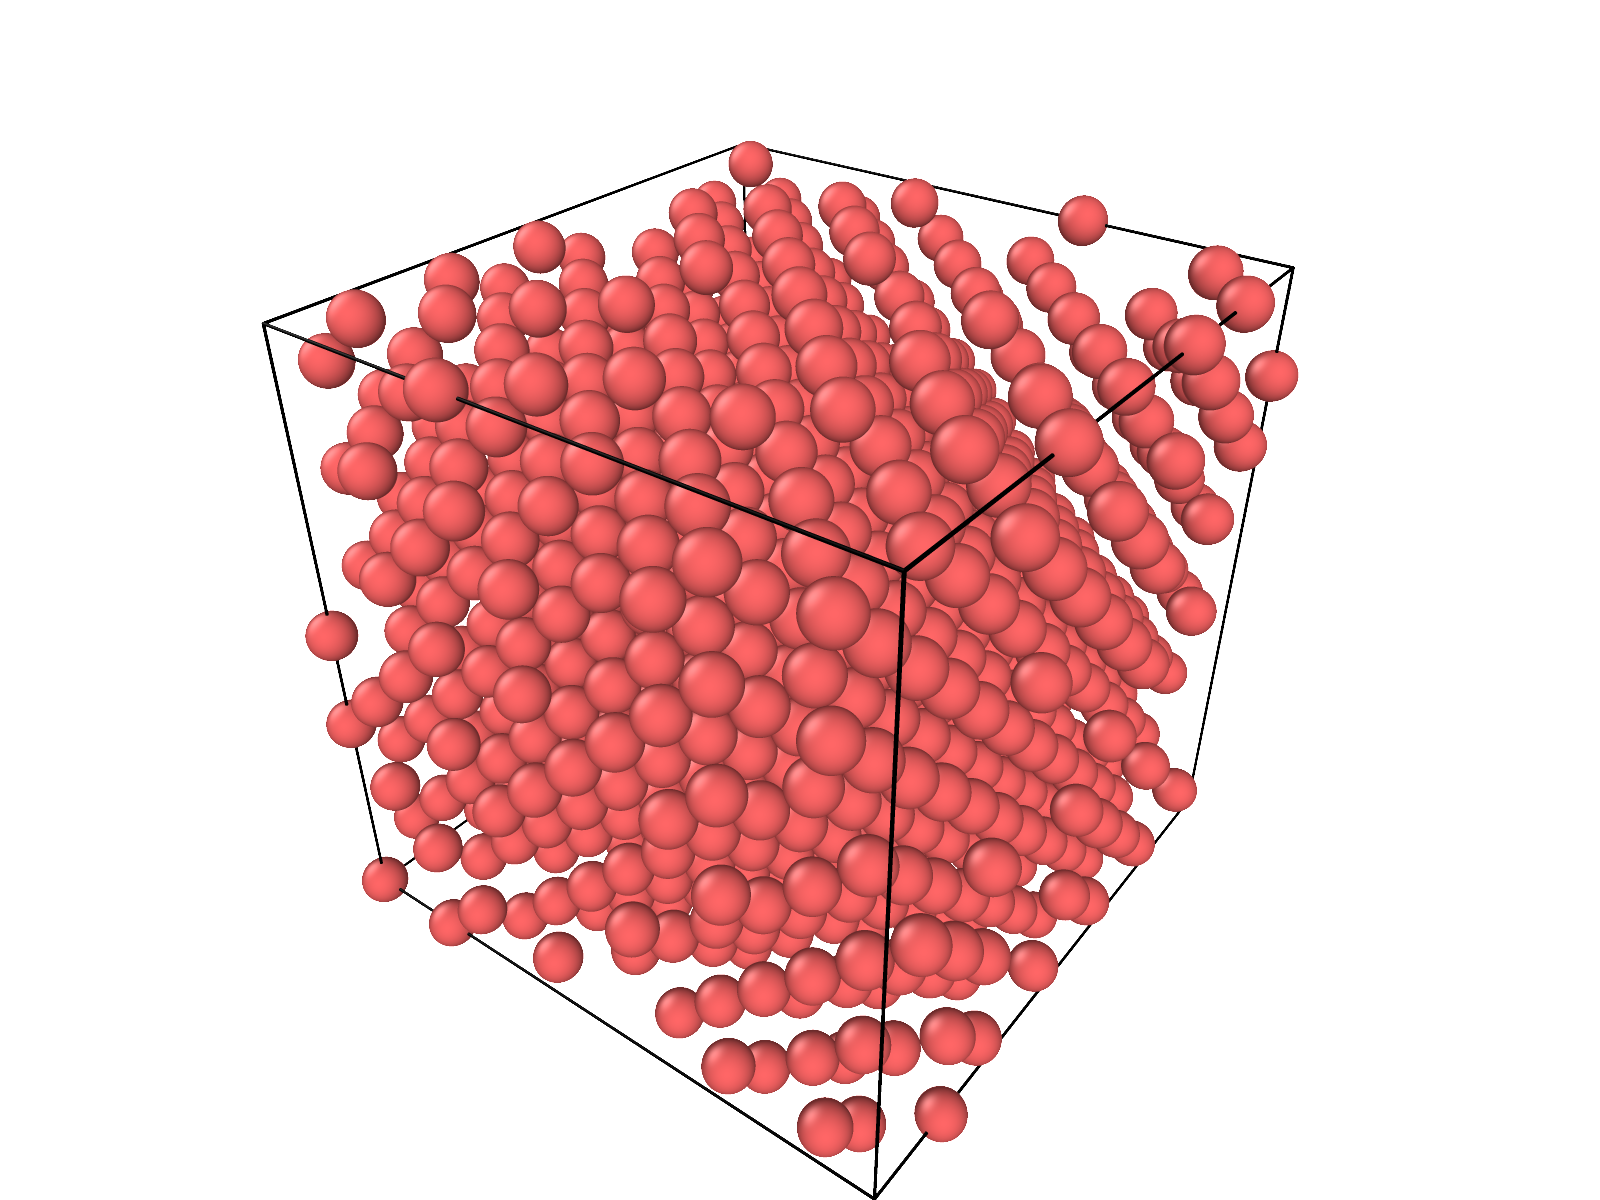
\includegraphics[width=\columnwidth]{lattice.png}
\caption{OVITO's rendering of the FCC lattice}
\label{ovito}
\end{figure}[ht]
\subsection{Parameters and units}
In the Lennard Jones model there are two numerical factor that need to be defined, $\epsilon$ and $\sigma$. The $\epsilon$ factor determines the energy scaling and the $\sigma$ is the distance at which the potential is zero. For Argon these values are taken to be:
\begin{align}
	\frac{\epsilon}{k_B} = 119.8\mathrm{K},  \sigma=3.405 \mathrm{Angstrom}.
\end{align}

The energy units in this project were carefully chosen to simplify the calculations.For these types of calculations it is convenient to define the Boltzmann constant equal to 1 so that the Temperature and Energy are interchangeable in magnitude. it is worth noting; we have used a unit conversion class to manage the units for the simulation.   

\subsection{Boundary Conditions}
Molecular Dynamics simulations are primarily limited by computational power. As such our simulations, which were run on personal computers, deal with a relatively small system. Since we want to generalize our results, based of simulations using ~1000 particles, to larger systems we used periodic boundary conditions. These say that the simulation occurs within a unit cell that has opposite sides connected. The good thing about this condition is that it doesn't require excessively large systems to determine how the atoms would move under certain conditions, this would allow for significantly reduced number of FLOPS being used for this simulation.
\subsection{Integration}
After the Initialization, We could run the actual simulation. First, the forces between each of the particles had to be calculated from the Lennard Jones potential. This took into consideration the periodic boundary conditions discussed above of course. Once the intermolecular forces were calculated the motion of each particle was calculated using the Verlet method, also described above.  

\subsection{OVITO}
After running the simulation, we used OVITO to help with the analysis of the data. OVITO is a visualization software that we used to interpret our results. It allowed us to see an animated rendition of the simulations which, in the context of molecular dynamics, gave a very tactile understanding of how the particles interacted within the potential\cite{ovito}. 

\section{Results}
First we evaluated a system with an initial temperature T = 300K to understand how the system equilibrated. We saw a drop in the energy up until INSERT TEMP and this held true in our further simulations.\\
ADD TABLE
\\
\subsection{Diffusion and the melting point}
The important result of this experiment is the temperature at which we see a phase transition. Since watching movies of the evolution of our simulation would have been inadequate for any kind of quantitative analysis we measured the diffusion constant to determine the location of the melting point. We did this with the Einstein relation:
\begin{equation}
D = \lim_{t \to \infty} \frac{\langle r^2(t) \rangle}{6t}
\end{equation}
Which we simply evaluate for large $t$ to ensure the system is in equilibrium. 
\begin{comment}
\begin{figure}
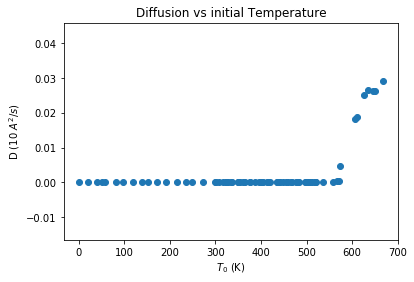
\includegraphics[width=\columnwidth]{t0vd.png}
\caption{This plots diffusion against initial temperature}
\label{initial}
\end{figure}
\end{comment}
\begin{figure}
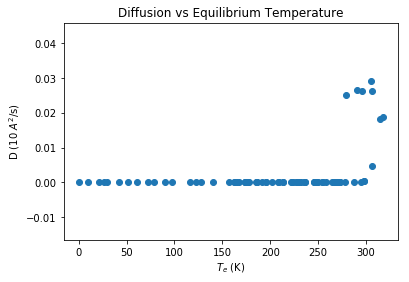
\includegraphics[width=\columnwidth]{tevd.png}
\caption{Diffusion against equilibrium temperature. note the effectively 0 value before 300K}
\label{eq}
\end{figure}
%\footnote{1}{All simulations were run with 10000 time steps and ~1000 particles}
Figure\ref{eq} shows the diffusion constant plotted as a function of  equilibrium temperature. We see that the Argon does not leave the solid state until roughly 300K after which the diffusion constant jumps without significant transition 
\subsection{Kinetic and Potential Energies}
We can estimate the energies of the system at this point using the equipartition theorem\cite{Kinetic}:
\begin{equation}
\langle E_K\rangle=\frac{3Nk_bT}{2}
\end{equation}
Where N is the number of atoms, k$_b$ is Boltzmann's constant and T is temperature in Kelvin. Since the only variable in this case is T, the plot of $\langle$E$_k\rangle$ would be proportional to T. Until the temperature reaches the transition temperature, it will grow linearly and them dip at that point, as can be seen by the following figure.
\begin{figure}
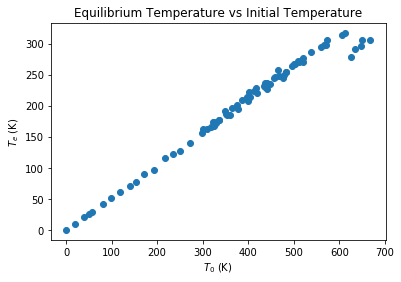
\includegraphics[width=\columnwidth]{tevt0.png}
\caption{By looking at the change in equilibrium temperature with respect to initial temperature we can see melting point and get a sense of the latent heat of the reaction.}
\label{tevt0}
\end{figure}
If we use equilibrium temperature we can, again, get a sense of the location of the melting point\ref{tevt0}. We see that the equilibrium temperatures drop off around 300K which is consistent with figure \ref{eq} 's location of the melting point. This tells us that there is a latent heat to this transition and that the transition can happen partially depending on the provided energy.


\section{Conclusions}
In its entirety, this model attempts to show how a lattice of atoms interact with one another through a given potential and initialization. For the case of Argon, it is not, since Argon requires additional components to the potential to make it accurate and the lattice structure. This is the reason why the melting point we got for this project was not correct, since we would have to adapt it specifically for Argon, such as changing the potential such that it is closer to what the actual potential is for argon in a lattice, instead of writing it for a general case, like was done here. If this was done, we would get the proper melting point and interactions between the atoms to reality.

\section{Future Additions}
In essence, this model is one of objects interacting with one another with a certain potential given initial conditions. This can really be expanded to anything, since all objects in the universe interact with other objects through a defined potential. We could probably model any macroscopic system given positions and possible potentials that an object interacts with. While systems which involves quantum mechanics would be a bit more difficult to model, but modifying the code and dealing with simple systems could cause this model to work to some extent. At this point, only one force is concerned, but the code could be modified to include multiple force.

\begin{thebibliography}{1}
\bibitem{morten github} Discussions and Lecture Slides on Ordinary Differential Equations. Morten Hjorth-Jensen. \url{https://compphysics.github.io/ComputationalPhysicsMSU/doc/pub/ode/html/ode-reveal.html}. GitHub. 
\bibitem{ovito}A. Stukowski, Visualization and analysis of atomistic simulation data with OVITO - the Open
Visualization Tool, Modelling Simul. Mater. Sci. Eng. 18 (2010), 015012 
\url{http://www.ovito.org.}
\bibitem{eleven}E.Leven et.al. "Escaping Lennard-Jones"
\url{https:
//github.com/erikalev/FYS3150/tree/master/Project%205}
\bibitem{Kinetic}Equation for average Kinetic Energy of a system in thermal equilibrium\url{https://en.wikipedia.org/wiki/Equipartition_theorem}
\bibitem{Mike's Github}Mike's Github, which contains the files that went into making the report \url{https://github.com/roosamic/roosa_PHY480MSU/tree/master/project4}
\end{thebibliography}
\end{document}
